\documentclass{minimal}
\usepackage{tikz}
\usepackage{color}
\usepackage[a4paper,margin=1cm,landscape]{geometry}
\usetikzlibrary{shapes,positioning}

\definecolor{namecolor}{RGB}{105,139,34}
\definecolor{elemcolor}{RGB}{234,232,170}

\begin{document}
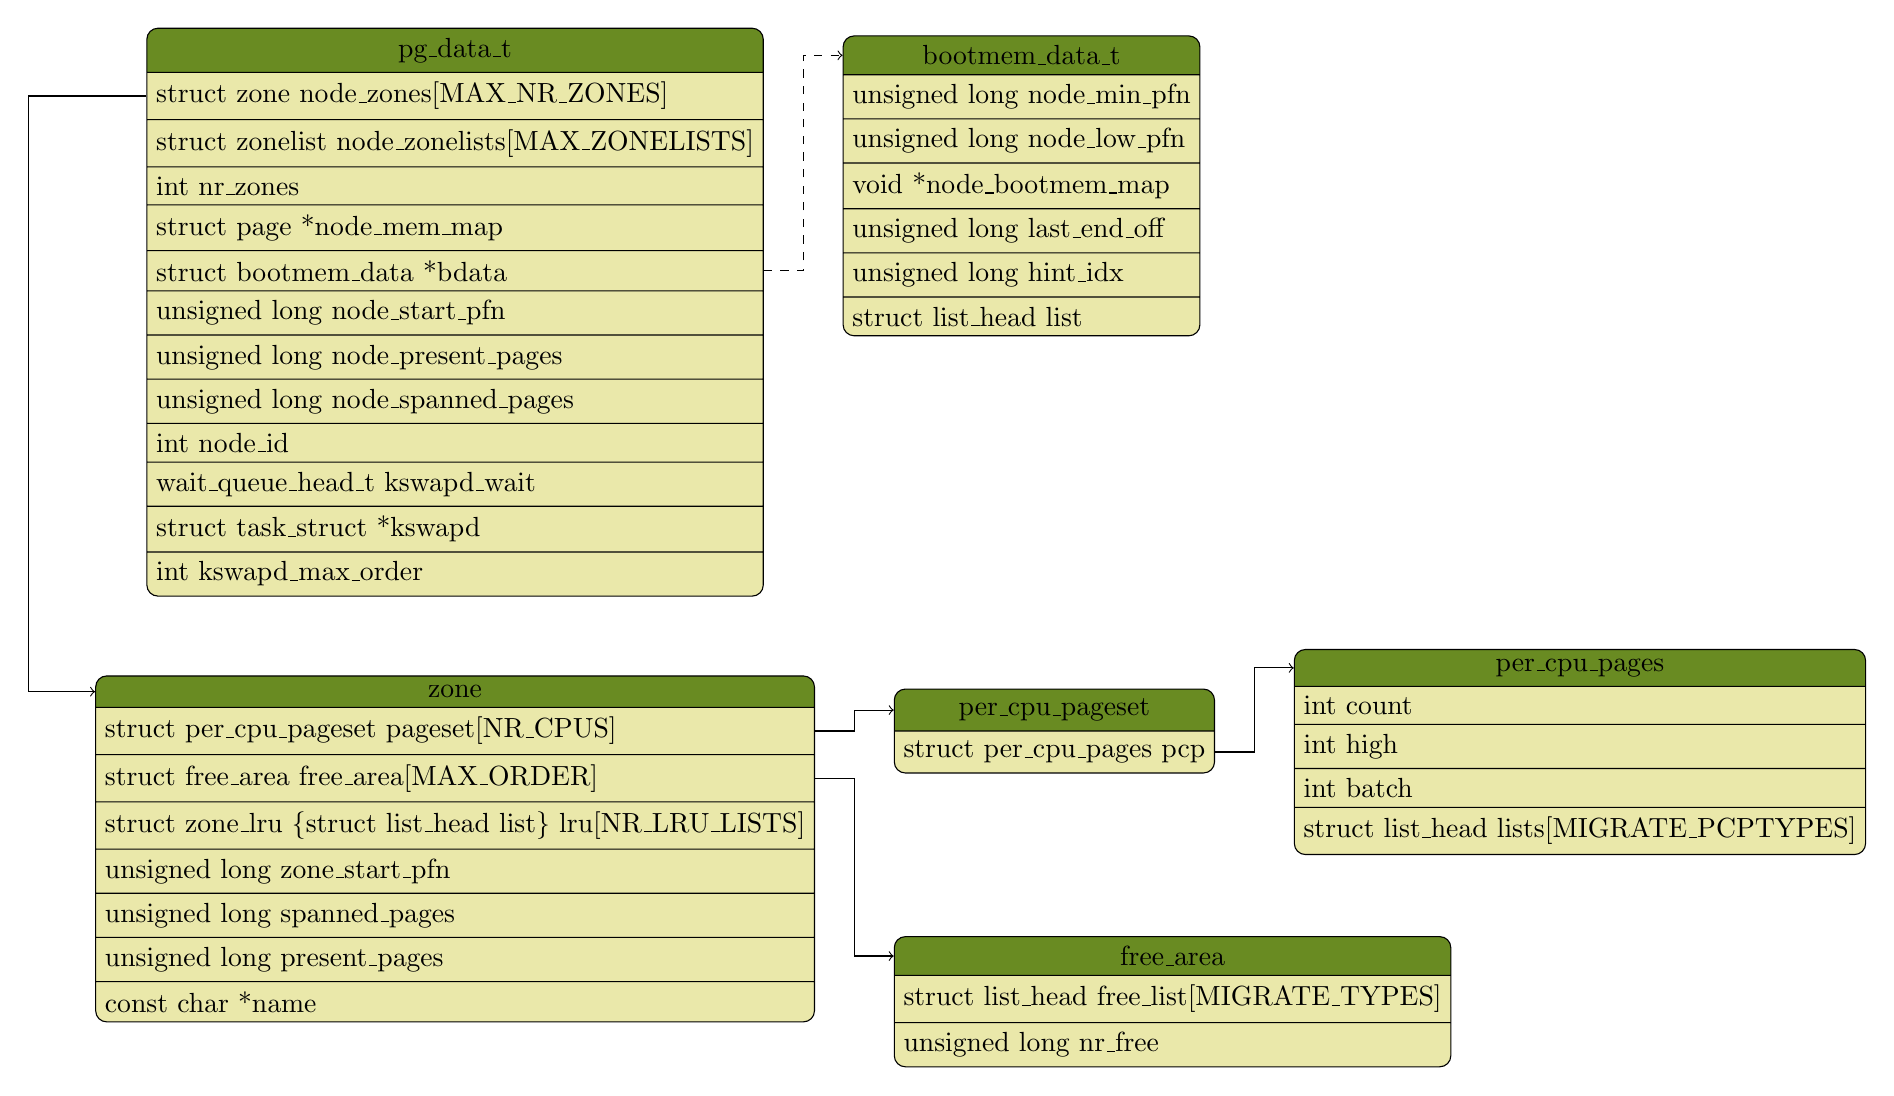
\begin{tikzpicture}[
    grow=right,
    element/.style={rectangle, rounded corners, rectangle split,
		rectangle split part align={center,left},
		rectangle split part fill={namecolor,elemcolor},
		draw}
    ]

\node[element, rectangle split parts=13] (pglistdata) {
	\nodepart{one}
	pg\_data\_t
	\nodepart{two}
	struct zone node\_zones[MAX\_NR\_ZONES]
	\nodepart{three}
	struct zonelist node\_zonelists[MAX\_ZONELISTS]
	\nodepart{four}
	int nr\_zones
	\nodepart{five}
	struct page *node\_mem\_map
	\nodepart{six}
	struct bootmem\_data *bdata
	\nodepart{seven}
	unsigned long node\_start\_pfn
	\nodepart{eight}
	unsigned long node\_present\_pages
	\nodepart{nine}
	unsigned long node\_spanned\_pages
	\nodepart{ten}
	int node\_id
	\nodepart{eleven}
	wait\_queue\_head\_t kswapd\_wait
	\nodepart{twelve}
	struct task\_struct *kswapd
	\nodepart{thirteen}
	int kswapd\_max\_order
};

\node[element, rectangle split parts=8] (zone) [below=of pglistdata] {
	\nodepart{one}
	zone
	\nodepart{two}
	struct per\_cpu\_pageset pageset[NR\_CPUS]
	\nodepart{three}
	struct free\_area free\_area[MAX\_ORDER]
	\nodepart{four}
	struct zone\_lru \{struct list\_head list\} lru[NR\_LRU\_LISTS]
	\nodepart{five}
	unsigned long zone\_start\_pfn
	\nodepart{six}
	unsigned long spanned\_pages
	\nodepart{seven}
	unsigned long present\_pages
	\nodepart{eight}
	const char *name
};

\node[element, rectangle split parts=2] (percpupageset) [right=of zone.two east] {
	\nodepart{one}
	per\_cpu\_pageset
	\nodepart{two}
	struct per\_cpu\_pages pcp
};

\node[element, rectangle split parts=5] (percpupages) [right=of percpupageset.two east] {
	\nodepart{one}
	per\_cpu\_pages
	\nodepart{two}
	int count
	\nodepart{three}
	int high
	\nodepart{four}
	int batch
	\nodepart{five}
	struct list\_head lists[MIGRATE\_PCPTYPES]
};

\node[element, rectangle split parts=3] (freearea) [right=of zone.eight east] {
	\nodepart{one}
	free\_area
	\nodepart{two}
	struct list\_head free\_list[MIGRATE\_TYPES]
	\nodepart{three}
	unsigned long nr\_free
};


\node[element, rectangle split parts=7] (bootmemdatat) [right=of pglistdata.four east] {
	\nodepart{one}
	bootmem\_data\_t
	\nodepart{two}
	unsigned long node\_min\_pfn
	\nodepart{three}
	unsigned long node\_low\_pfn
	\nodepart{four}
	void *node\_bootmem\_map
	\nodepart{five}
	unsigned long last\_end\_off
	\nodepart{six}
	unsigned long hint\_idx
	\nodepart{seven}
	struct list\_head list
};

\draw[->] (pglistdata.two west) -- ++(left:15mm) |- (zone.one west);
\draw[->,dashed] (pglistdata.six east) -- ++(right:5mm) |- (bootmemdatat.one west);
\draw[->] (zone.two east) -- ++(right:5mm) |- (percpupageset.one west);
\draw[->] (zone.three east) -- ++(right:5mm) |- (freearea.one west);
\draw[->] (percpupageset.two east) -- ++(right:5mm) |- (percpupages.one west);

\end{tikzpicture}
\end{document}
